\documentclass{article}
\usepackage[utf8]{inputenc}
\newcommand{\ii}{{\bf i}}
\newcommand{\jj}{{\bf j}}
\newcommand{\kk}{{\bf k}}
\newcommand{\id}{{\bf 1}}
\newcommand{\hur}{\frac{\id+\ii+\jj+\kk}{2}}%The "Hurwitz point"
\newcommand{\hurwitz}{\Z\left[\hur,\ii,\jj,\kk\right]}%The set of Hurwitz integers
\usepackage{wrapfig}
\usepackage{calligra}
\usepackage[utf8]{inputenc}
\usepackage[dvips]{graphicx}
\usepackage{a4wide}
\usepackage{amsmath}
\usepackage{euscript}
\usepackage{amssymb}
\usepackage{amsthm}
\usepackage{amsopn}
\usepackage[colorinlistoftodos]{todonotes}
\usepackage{graphicx}
\usepackage[T1]{fontenc}
\newcommand\mybar{\kern1pt\rule[-\dp\strutbox]{.8pt}{\baselineskip}\kern1pt}

\usepackage{ulem}
\usepackage{xcolor}
\newcommand{\cs}[1]{\color{blue}{#1}\normalcolor}

%Matrix commands
\newcommand{\ba}{\begin{array}}
\newcommand{\ea}{\end{array}}
\newcommand{\bmat}{\left[\begin{array}}
\newcommand{\emat}{\end{array}\right]}
\newcommand{\bdet}{\left|\begin{array}}
\newcommand{\edet}{\end{array}\right|}
\newcommand{\inv}[1]{#1^{-1}}

%Environment commands
\newcommand{\be}{\begin{enumerate}}
\newcommand{\ee}{\end{enumerate}}
\newcommand{\bi}{\begin{itemize}}
\newcommand{\ei}{\end{itemize}}
\newcommand{\bt}{\begin{thm}}
\newcommand{\et}{\end{thm}}
\newcommand{\bp}{\begin{proof}}
\newcommand{\ep}{\end{proof}}
\newcommand{\bprop}{\begin{prop}}
\newcommand{\eprop}{\end{prop}}
\newcommand{\bl}{\begin{lemma}}
\newcommand{\el}{\end{lemma}}
\newcommand{\bc}{\begin{cor}}
\newcommand{\ec}{\end{cor}}
\newcommand{\lcm}{\mbox{lcm}}
\newcommand{\defn}{\fbox{definition}}
\newcommand{\prop}{\fbox{proposition}}
\newcommand{\stab}{\mbox{stab}}
\newcommand{\Aut}{\mbox{Aut}}
\newcommand{\orb}{\mbox{orb}}

\newcommand{\norm}{\righttriangle}

\newcommand{\and}{\wedge}
\newcommand{\or}{\vee}



%sets of numbers
\newcommand{\N}{\mathbb{N}}
\newcommand{\Z}{\mathbb{Z}}
\newcommand{\Q}{\mathbb{Q}}
\newcommand{\R}{\mathbb{R}}

\newcommand{\topT}{\mathcal{T}}
\newcommand{\standtop}{\mathcal{T}_{STD}}
\newcommand{\cc}{\mathcal{C}}


\title{Topology}
\author{August bergquist}


\begin{document}
\fbox{lemma} Given collections of sets $\{X_\alpha\}_{\alpha\in A}$ and $\{Y_{\beta}\}_{\beta\in B}$, 
$$ $$

\fbox{Theorem 3.3} Suppose that $X$ is a set and $\mathcal{B}$ is a collection of subsets of $X$. Then $\mathcal{B}$ is a basis for some topology on $X$ if and only if
\begin{enumerate}
    \item each point of $X$ is in some element of $\mathcal{B}$, and
    \item if $U$ and $V$ are sets in $\mathcal{B}$ and $p$ is a point in $U\cap V$, there is a set $W$ in $\mathcal{B}$ such that $p\in W \subseteq (U\cap V)$
\end{enumerate}

\fbox{proof} 
\begin{itemize}
    \item[$\Rightarrow$] Suppose that $\mathcal{B}$ is a basis for some topology $\topT$ on $X$. Let $p$ be an arbitrary point of $X$. Since $X$ itself must be in $\topT$ as follows from the definition of a topology, it follows by definition of a basis that $X = B_1\cup \dots\cup B_n$ for elements $B_1,\dots,B_n\in \mathcal{B}$. Then by definition of unions, $x\in B_i$ for some $B_i\in \mathcal{B}$ being unioned over. Since $x$ was arbtirary in $X$, it follows that every point of $X$ is in some member of $\mathcal{B}$. Now we suppose that $U$ and $V$ are sets in $\mathcal{B}$ and that $p$ is some point in $U\cap V$. Since elements of a basis are also open sets, $U$ and $V$ are open, and since the intersection of open sets in a topology must be open, it follows that $U\cap V$ is open. Since $U\cap V$ is open, and since by supposition $\mathcal{B}$ is a basis, it follows that $U\cap V$ must be the union of elements $B_1,\dots,B_n\in \mathcal{B}$ (these are now distinct from the ones instantiated above). Since $p\in U\cap V = B_1\cup \dots \cup B_n$, it follows by definition of the union that $B_i$ for one of these $B$'s. Furthermore, using rules of set theory, we know that $B_i \susbeteq B_1\cup \dots \cup B_i \cup \dots\cup B_n = U\cap V$, and noting that $B_i$ is open since its an element of $\mathcal{B}$, it follows that there is a set in $\mathcal{B}$, namely $B_i$, such that $p\in B_i\subseteq U\cap V$.
    \item[$\Leftarrow$] Now we suppose that (a) every point in $X$ is in some element in $\mathcal{B}$ and (b) for any elements $U$ and $V$ in $\mathcal{B}$, if $p\in U\cap V$ there is a set $W\in \mathcal{B}$ such that $p\in W\subseteq (U\cap V)$. We want to show that there is some topology $\mathcal{T}$ on $X$ for which $\mathcal{B}$ is a basis.\\

    Consider the set of all unions of elements in $\mathcal{B}$, call it $\mathcal{T}$. We will show that, given suppositions $(a)$ and $(b)$, $\mathcal{T}$ is a topology on $X$.
    \begin{enumerate}
        \item To show that $\emptyset\in \mathcal{T}$ consider the empty union.
        \item To show that $X\in \mathcal{T}$, consider the union of all elements in $\mathcal{B}$, $\bigcup_{B\in \mathcal{B}}B$. We now want to show that $ \bigcup_{B\in \mathcal{B}}B = X$
        \begin{itemize}
            \item[$\subseteq$] Since each $B$ is a subset of $X$ by construction, we know that $ \bigcup_{B\in \mathcal{B}}B$ must be a subset of $X$
            \item[$\supseteq$] Let $x$ be an arbitrary element in $X$. Since by supposition (a) we know that there is some $B\in \mathcal{B}$ such that $x\in B$, it follows that $x\in \bigcup_{B\in \mathcal{B}}B$, hence $X\susbeteq \bigcup_{B\in \mathcal{B}}B$.
        \end{itemize}
        \item Now suppose that $U$ and $V$ are elements of $\mathcal{T}$. Then by construction of $\mathcal{T}$, $U = A_1\cup \dots\cup A_n$ and $V = B_1\cup \dots \cup B_m$ for elements $A_1,\dots,A_n,B_1,\dots,B_m\in \mathcal{B}$. I'm a bit stuck here, any ideas?
        \item Consider an arbitrary union of sets on $\topT$, $\bigcup U$. Since each $U$ is itself a union of elements in $\mathcal{B}$, it follows that so is $\bigcup U$.
    \end{enumerate}
\end{itemize}

\fbox{exercise 3.4} Check that the basis for the lower limit topology (the set of all subsets of $\R$ of the form $[a,b)$ ) is a basis. \\

\fbox{solution} We don't need to show that it is the basis for any specific topology, only for any old one. We can use the theorem we just proved.\\

Let $a$ be an arbitrary real number. Consider the set $[a,a+1)$, which is in the lower limit topology, and contains $x$. Hence every element $a\in \R$ is in member of the lower limit topology.\\

Let $U$ and $V$ be elements of the lower limit topology. By construction of the lower limit topology $U = [a,b)$ and $V = [c,d)$ for $a,b,c,d\in \R$. If either sets are empty (that is, if $a\ge b$ or $c\ge d$), then their intersection is empty and the second requirement of theorem 3.3 is vacuously true. Suppose then that $a < b$ and $c < d$. Then the only case where their intersection will be non-empty is when there is some overlap between the intervals. If its empty, then as we've shown, we're done. If they're not, $b < c$ or $d < b$. WLOG suppose $b < c$. Then the intersection of these two intervals forms $[b,d)$, which is another element of the basis for the lower limit topology. Since it is, and since $[b,d)$ is the intersection and must be a susbet of itself, the second requirement of theorem 3.3 is satisfied in this case as well.
\begin{figure}[htbp]
\centerline{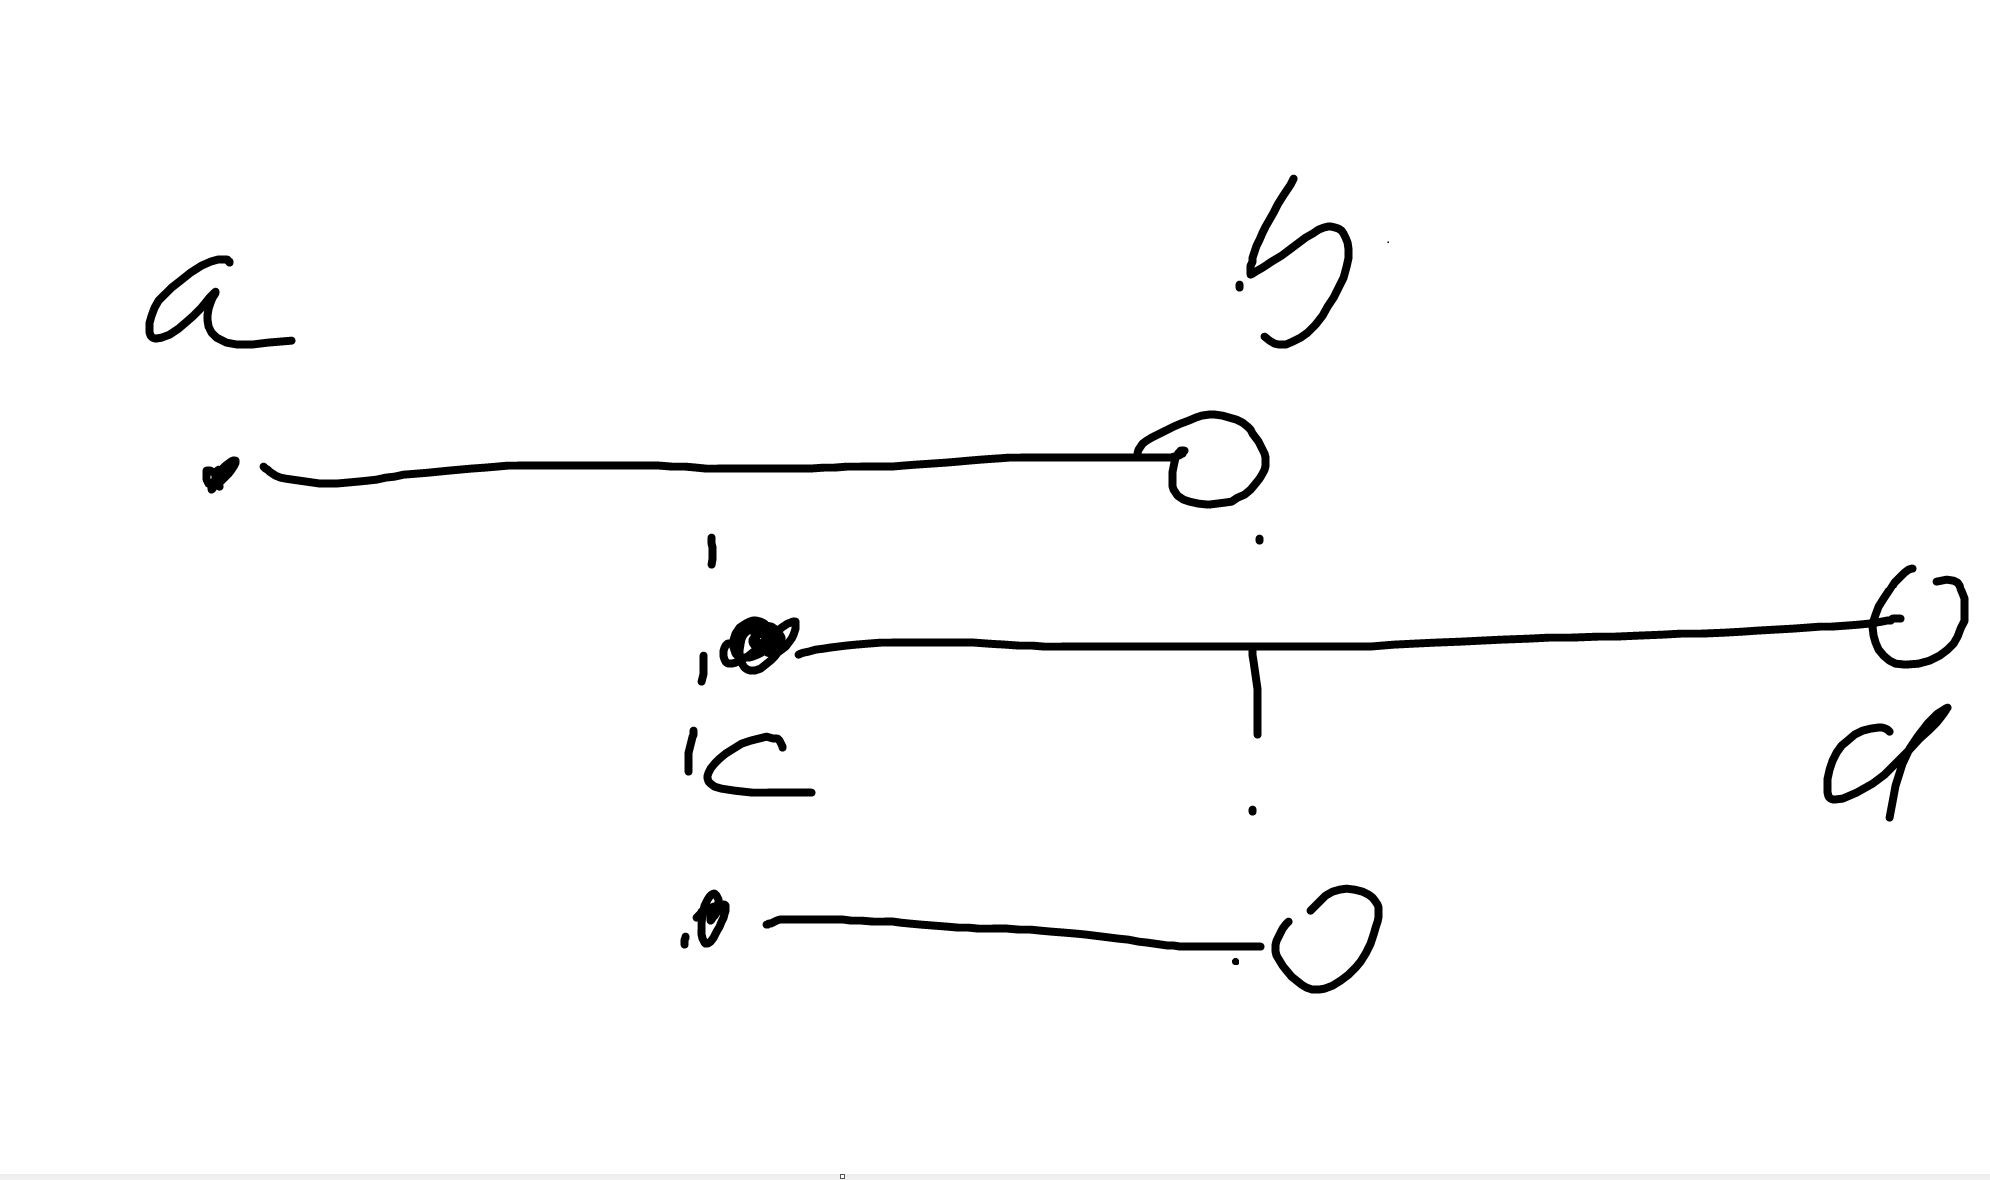
\includegraphics[scale=0.5]{notebook/intervals.png}}
\caption{what this proof looks like in $\R^2$}
\label{fig}
\end{figure}
\\


\newpage

\fbox{exercise 3.14} Show that $\R$ with the standard topology has a subbasis $\mathcal{S}$ consisting of rays $\{x| s< a \mbox{ for some } a\in \R\}$ and $\{x| s> a \mbox{ for some } a\in \R\}$
\\

\fbox{solution} From exercise 3.2 we know that $\mathcal{B}_1 = \{(a,b) : a,b\in \Q\}$ is a basis for the standard topology on $ \R$, and also that $\mathcal{B}_2= \{(a,b): a,b\in \R-\Q\}$ is a basis for $\standtop$ as well. Since all that is required for a basis is that each of its elements be open in the topology, and that each element of the topology is a union of elements in the basis, we know that the union of two bases for a topology is also a basis. Adding in the empty set won't hurt either. Hence $\mathcal{B} = \{(a,b) : a,b\in \R\}\cup\{\emptyset\}$ is a basis for the standard topology on $\R$.\\

Now we want to show that $\mathcal{B}$ is the set of all finite intersections of elements in $\mathcal{S}$, which will mean that $\mathcal{S}$ generates the basis $\mathcal{S}$, which in turn is a basis for $\standtop$, which will show that $\mathcal{S}$ is a subbasis of $\standtop$.\\

Its easier to draw pictures to show how in any case the intersection will be in $\mathcal{B}$:
\begin{figure}[htbp]
\centerline{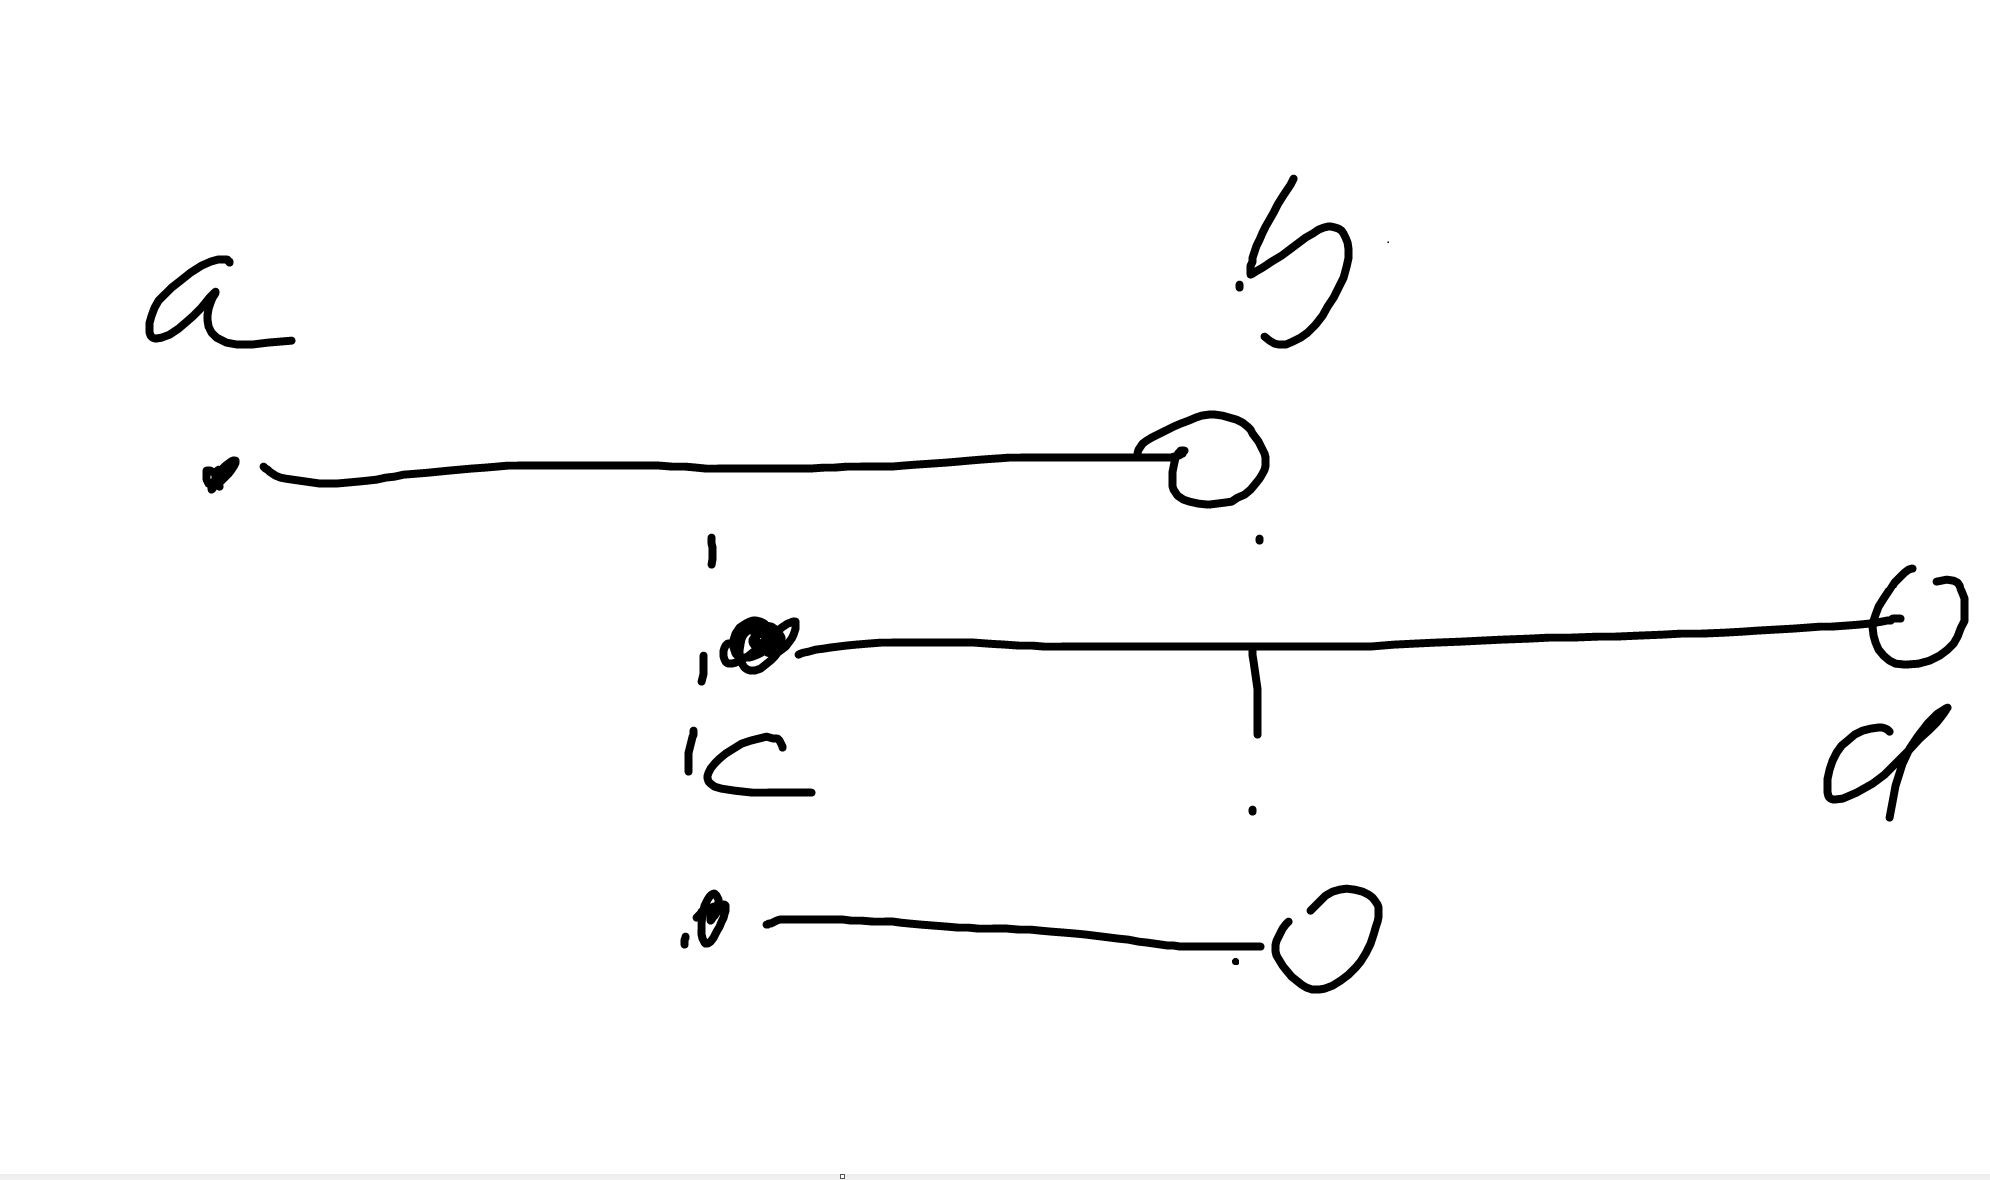
\includegraphics[scale=0.5]{notebook/intervals.png}}
\caption{what this proof looks like in $\R^2$}
\label{fig}
\end{figure}
\\





\\

\fbox{Theorem 3.25} Let $X$ be a set and let $\topT$ be a topology on $X$. Then the set $\topT_Y = \{U : U = V\cap Y \mbox{ for some } V\in \TopT \}$ is a topology on $X$.\\

\fbox{proof} Let $Y$ by an arbitrary subset of $X$. To show that $\topT_Y$ is a topology on $Y$, we need to show that it satisfies that topology axioms.
\begin{enumerate}
\item Since $\emptyset\in \topT$ as follows from $\topT$ being a topology on $X$, we know that $\emptyset = \emptyset \cap V \in \topT_Y$ as follows by construction of $\topT_Y$.
\item Since $X\in \topT$ by definition of a topology, and since $Y\cap X = Y$ because $Y\subseteq X$, it follows by definition that $Y \in \topT_Y$.
\item Let $A$ and $B$ be arbitrary elements of $\topT_Y$. Then by construction of $\topT_Y$ it follows that $A = U\cap Y$ and $B = V\cap Y$ for elements $U,V\in \topT$. Hence by substitution and rules of set theory we know that $A\cap B = (U\cap Y)\cap (V\cap Y) = (U\cap V)\cap Y$. Since $\topT$ is a topology and $U,V\in \topT$ we know by definition of a topology that $U\cap V\in \topT$. Hence by definition of $\topT_Y$ it follows that $A\cap B\in \topT_Y$.
\end{enumerate}


\fbox{exercise 3.26} Consider $Y = [0,1)$ as a subspace of $\R_{std}$. In $Y$ is the set $[1/2,2)$ open, closed, neither, or both.\\

\fbox{solution} First, we note that $\topT_Y$ will be intersections of $[0,1)$ and open sets in the standard topology. There's no way to get $[1/2,1)$ in this way, as it would require $1/2$ to be in an open set, but $1/2 + \epsilon$ cannot be in that open set for some $\epsilon> 0$, for if it were, $1/2$ would not be the smallest member of $[1/2, 1)$. So it isn't closed.\\

Consider any point outside of $[0,1) - [1/2,1) = [0,1/2]$. This set cannot be open, for the open set would have to include some interval ending at and including $1/2$, but there could be no margin $\epsilon$. Since the set compliment of $[1/2,1)$ is not open, $[1/2,1)$ cannot be closed by theorem 2.14.
\end{document}